\documentclass[utf8, xcolor=dvipsnames]{beamer}
% \usetheme{Frankfurt} % Boadilla - Ilmenau

\usepackage{graphicx}
\usepackage{setspace}
\usepackage{csquotes}
\usepackage{changepage}
\usepackage{color}
\usepackage[colorlinks = TRUE, allcolors = blue]{hyperref}
\useinnertheme{rectangles}
\usepackage{tikz}
\usetikzlibrary{graphs}
\usetikzlibrary{decorations.pathreplacing}

% \setbeamercovered{transparent}
\setbeamercolor{title}{bg=Blue, fg=white}
\setbeamercolor{title_int}{bg=white, fg=Blue}
\setbeamertemplate{navigation symbols}{}
\setbeamertemplate{itemize items}[circle]
\setbeamertemplate{blocks}[default]
\setbeamertemplate{headline}[default]
\setbeamertemplate{section in head}{}
\setbeamertemplate{subsection in head}{}
\setbeamercolor{section in foot}{fg=Blue, bg=white}
\setbeamercolor{subsection in foot}{fg=Blue, bg=white}
\setbeamercolor{frametitle}{fg=Blue, bg=white}
\setbeamercolor{footlinecolor}{bg=white,fg=Blue}
\useoutertheme[compress]{miniframes}

\makeatother
\setbeamertemplate{footline}
{%
  \leavevmode%
  \hbox{
  \begin{beamercolorbox}[wd=\paperwidth,ht=2.5ex,dp=1.125ex,leftskip=.3cm,rightskip=.3cm plus1fil]{footlinecolor}%
    \usebeamerfont{author in head/foot}
    \insertshorttitle\hfill\insertshortauthor\hfill\insertshortdate\hfill\insertframenumber/\inserttotalframenumber
  \end{beamercolorbox}}%
  \vskip0pt%
}
\setbeamertemplate{headline}[default]
{%
    \def\beamer@entrycode{\vspace*{0pt}}
}
\makeatletter

\title[War, peace, and political violence]{War, peace, and political violence:\\Nationalism}
\author[Francisco Villamil]{Francisco Villamil}
\date[UC3M / Fall 2022]{Fall 2022\\Universidad Carlos III de Madrid}

\begin{document}


\begin{frame}
  \titlepage
\end{frame}

\begin{frame}
\frametitle{Nations and Nationalism}
\centering

\begin{itemize}[<+->]
  \item Rise of nationalism in the late 18th/early 19th centuries, and its relationship with political violence
  \item[]
  \item Nations: `imagined communities' of people with a sense of commonality based on linguistic, territorial, ethnic, or religious traits
  \item Nations $=$ fully mobilized ethnic groups, claims of statehood
  \begin{itemize}
    \item Some ethnic groups do not claim statehood, some nations are multi-ethnic (Switzerland)
  \end{itemize}
  \item Nationalism: political ideology, congruence between units of political sovereignty and nations
\end{itemize}

\end{frame}

\begin{frame}
\frametitle{Emergence of nationalism}
\centering

\begin{itemize}[<+->]
  \item American Revolution
  \item Independence movements in Spanish South America
  \item French Revolution
  \item Full development during 19th century
\end{itemize}

\end{frame}

\begin{frame}
\frametitle{Why it happened}
\centering

\begin{itemize}[<+->]
  \item Several theories explaining the rise of nationalism
  \item Economic modernization (Ernest Gellner)
  \begin{itemize}
    \item Industrial revolution, homogenous workforce, standardized education
  \end{itemize}
  \item Rise of cultural modernization (Benedict Anderson)
  \begin{itemize}
    \item Mass literacy in vernacular languages, rise of printing press capitalism, legacies of administrative divisions
  \end{itemize}
  \item Shift to direct rule (Charles Tilly, Michael Hechter, etc)
  \begin{itemize}
    \item Homogenous state administration, nation-building policies, etc
  \end{itemize}
  \item Other theories: Meyer's world polity theory, ...
\end{itemize}

\end{frame}

\begin{frame}
\frametitle{The French Revolution and warfare}
\centering

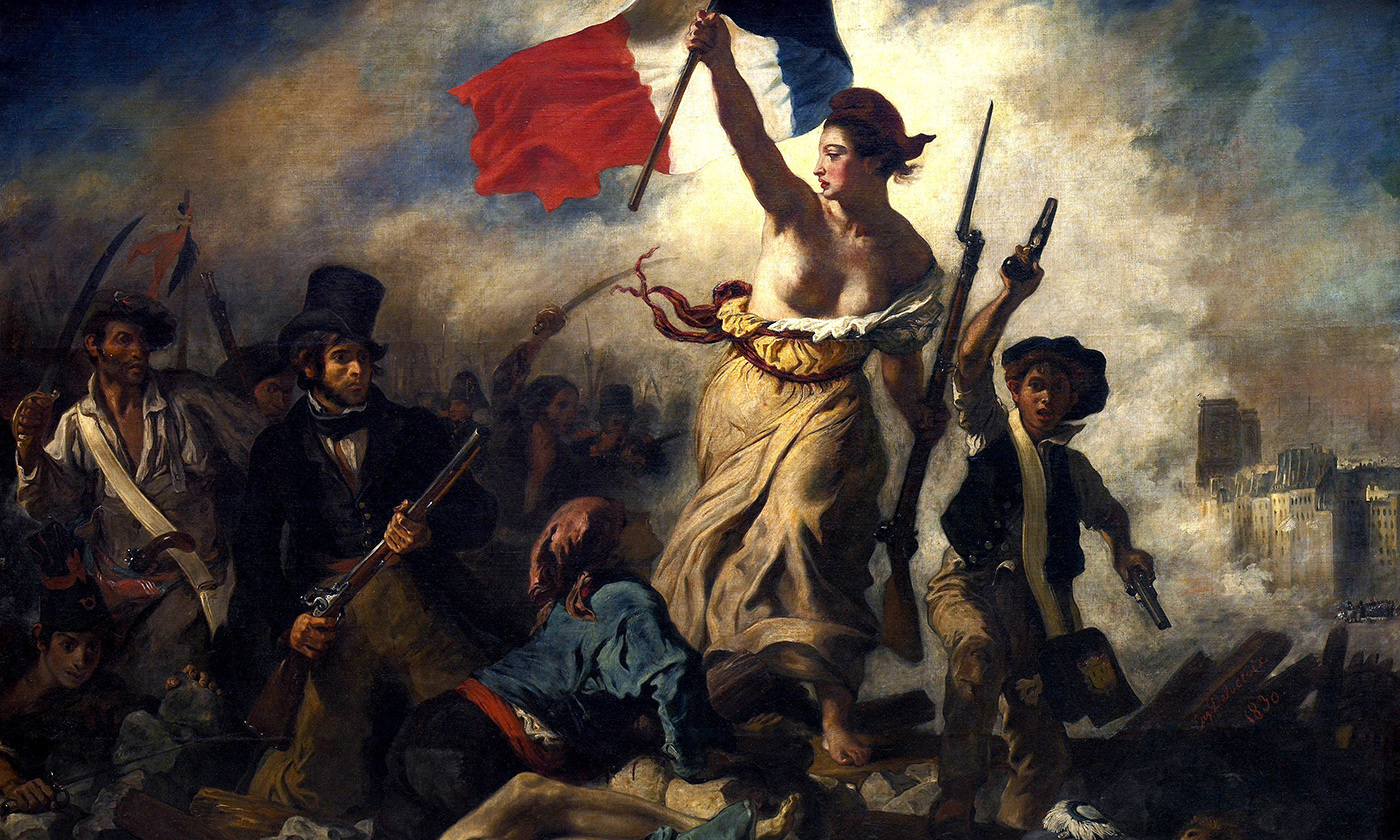
\includegraphics[width = 0.6\textwidth]{img/delacroix}

% Delacroix (1930)

\vspace{15pt}

\begin{quote}
  {\small ``in 1793 a force appeared that beggared all imagination. Suddenly war again became the business of the people---a people of thirty millions, all of whom considered themselves to be citizens. (...) the full weight of the nation was thrown into the balance.''}
\end{quote}

{\small (Clausewitz, \textit{On War})}

\end{frame}

\begin{frame}
\frametitle{What happened in international politics?}
\centering

\begin{itemize}[<+->]
  \item Main idea: Nationalist systems change after French Revo
  \item Gilpin's typology of international change
  \begin{itemize}
    \item Interaction change (the way states relate to each other)
    \item Systemic change (`Waltzian' balance, etc)
    \item Systems change (the very \textit{nature} of the units)
  \end{itemize}
  \item Previous change: Westphalia and the territorial systems change
  \item Explaining impact on inter-state warfare at a global level: \textit{historical} patterns of war
  % \item[]<1-> {\footnotesize \textit{Source:} Cederman, Camber Warren, and Sornette (\textit{International Organization}, 2011)}
 \end{itemize}

\end{frame}

\begin{frame}
\frametitle{Territorial systems change}
\centering

\begin{itemize}[<+->]
  \item Usual date: Peace of Westphalia in 1648
  \item Emergence of the modern state
  \item New scenario: internal monopoly of violence \& territorial sovereignty
  \item Direct, coercive methods of resource extraction
  \begin{itemize}
    \item Different from indirect rule, where tax/resource collection and coercion are outsourced
  \end{itemize}
  \item New warfare: Standing armies, better weapons, larger wars, ...
\end{itemize}

\end{frame}

\begin{frame}
\frametitle{Nationalist systems change}
\centering

\begin{itemize}[<+->]
  \item Usual date: French Revolution
  \item Birth of the modern \textit{nation}, the imagined communities
  \item New technology of statecraft: nation-building through mass schooling, mass mobilization, popular sovereignty, etc
  \begin{itemize}
    \item Remember previous technologies of statecraft: earliest states and the `domestication' of humans (Scott), Early Modern Europe and the emergence of direct rule (Tilly), etc
  \end{itemize}
  \item Loyalty replaces coercion, mass popular armies replace professional armies
  \begin{itemize}
    \item That's why Clausewitz spoke of a new ``force ... that beggared all imagination'', and added that ``nothing now impeded the vigor with which war could be waged''
  \end{itemize}
\end{itemize}

\end{frame}

\begin{frame}
\frametitle{Did the French Revolution change warfare?}
\centering

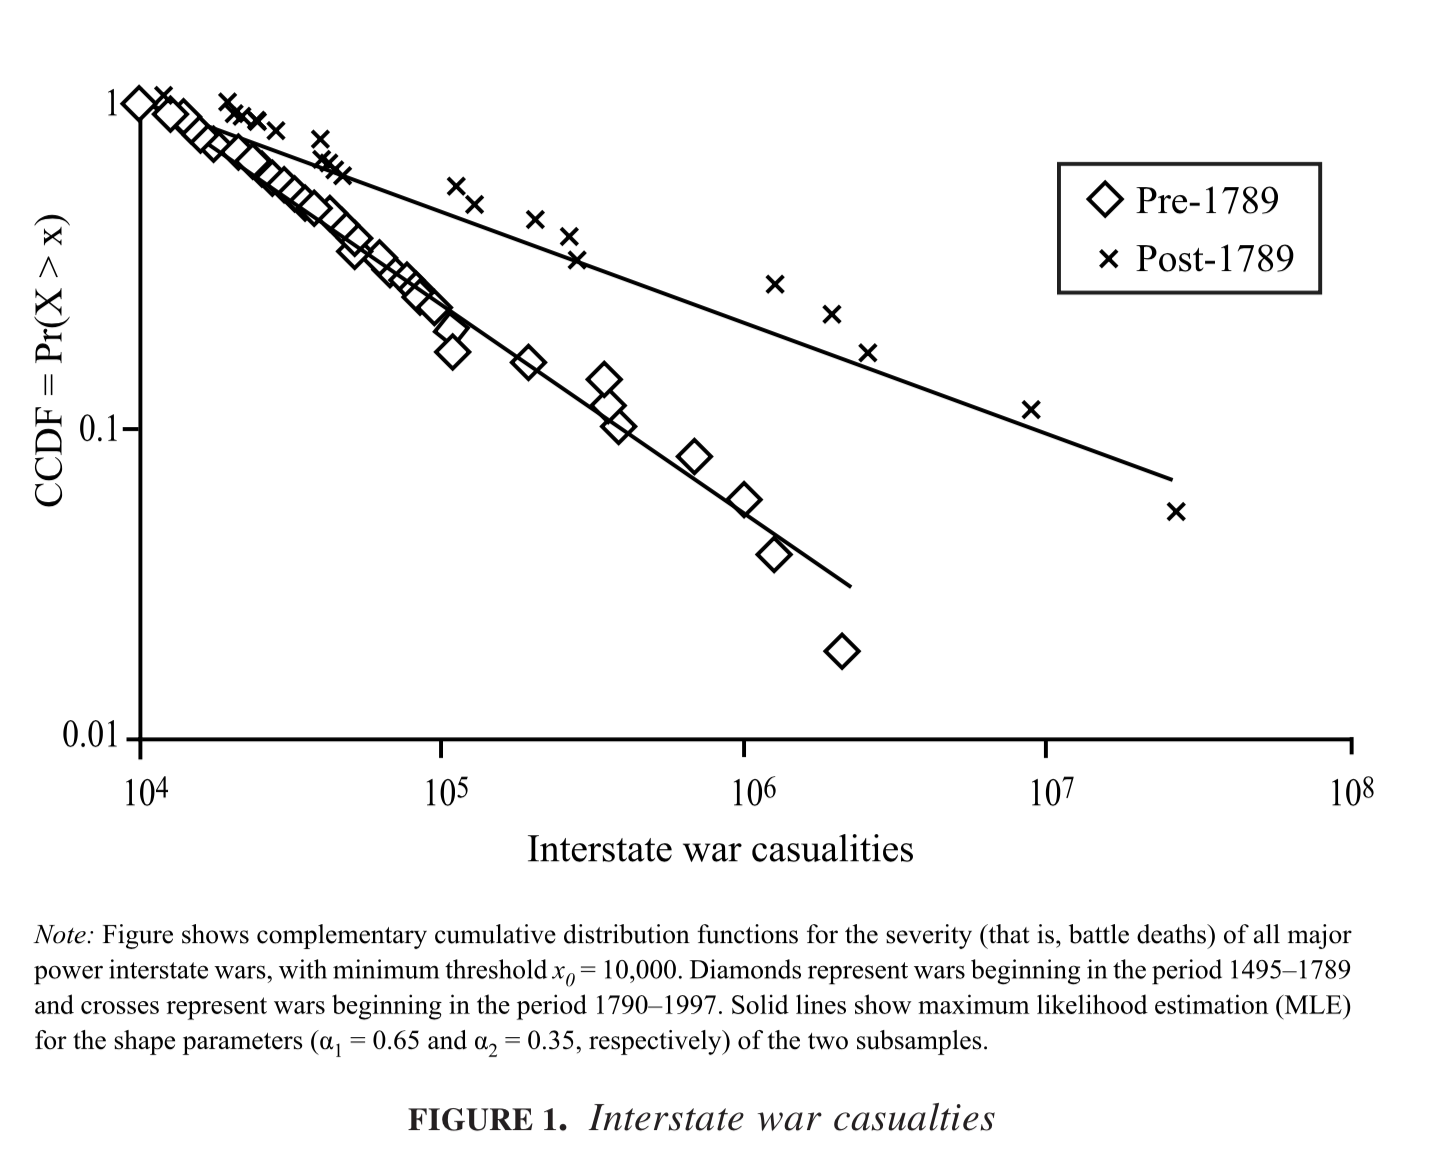
\includegraphics[width = 0.85\textwidth]{img/cederman_et_al_fig1}

{\scriptsize \textit{Source:} Cederman, Camber Warren, \& Sornette (2011)}

\end{frame}

\begin{frame}
\frametitle{Did the French Revolution change warfare?}
\centering

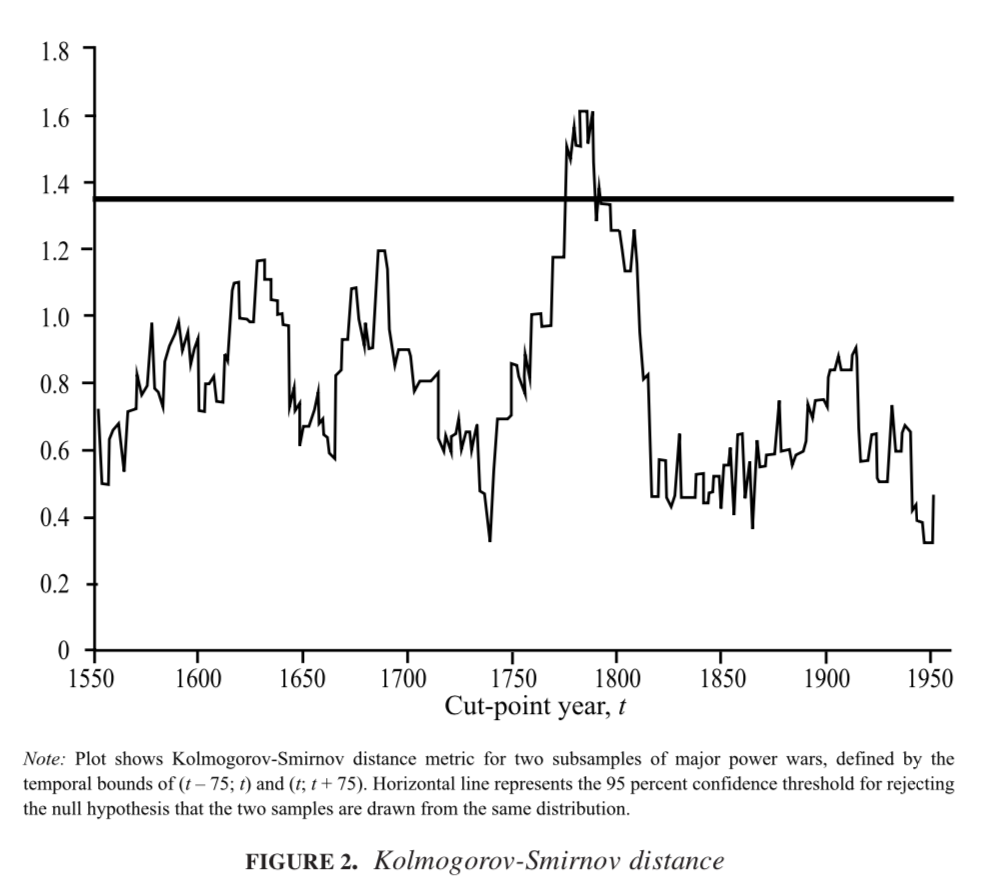
\includegraphics[width = 0.75\textwidth]{img/cederman_et_al_fig2}

{\scriptsize \textit{Source:} Cederman, Camber Warren, \& Sornette (2011)}

\end{frame}

\begin{frame}
\frametitle{Major institutional changes and war}
\centering

\begin{itemize}[<+->]
  \item Usual studies of war occurrence focus on specific wars, and the conditions leading to each war onset
  \item Can we think of a global explanations for historical patterns of warfare over the long run?
  \item Looking at global institutional patterns: how polities are organized and how they changed
  \item Claim: likelihood of wars (both interstate and civil wars) is higher in periods of institutional change, in particular, the main two processes taking place in the last 200 years: incorporation into empires and formation of nation-states
  % \item \textit{Source:} Wimmer \& Min (\textit{American Sociological Review}, 2006)
\end{itemize}

\end{frame}

\begin{frame}
\frametitle{Empires \& nation-states}
\centering

\begin{itemize}[<+->]
  \item Two main competing models of state-building since the French Revolution
  \item Empires
  \begin{itemize}
    \item Centralized bureaucratic government, core region ruling over the periphery, claims to universal legitimacy (ideologies, religion), ...
  \end{itemize}
  \item Nation-states
  \begin{itemize}
    \item Also centralized bureaucracy, but uniform rule over a territory and claims to popular sovereignty
  \end{itemize}
  \item Displacing previous institutional set-ups: absolutist kingdoms, city states, feudalism...
\end{itemize}

\end{frame}

\begin{frame}
\frametitle{Empires \& nation-states}
\centering

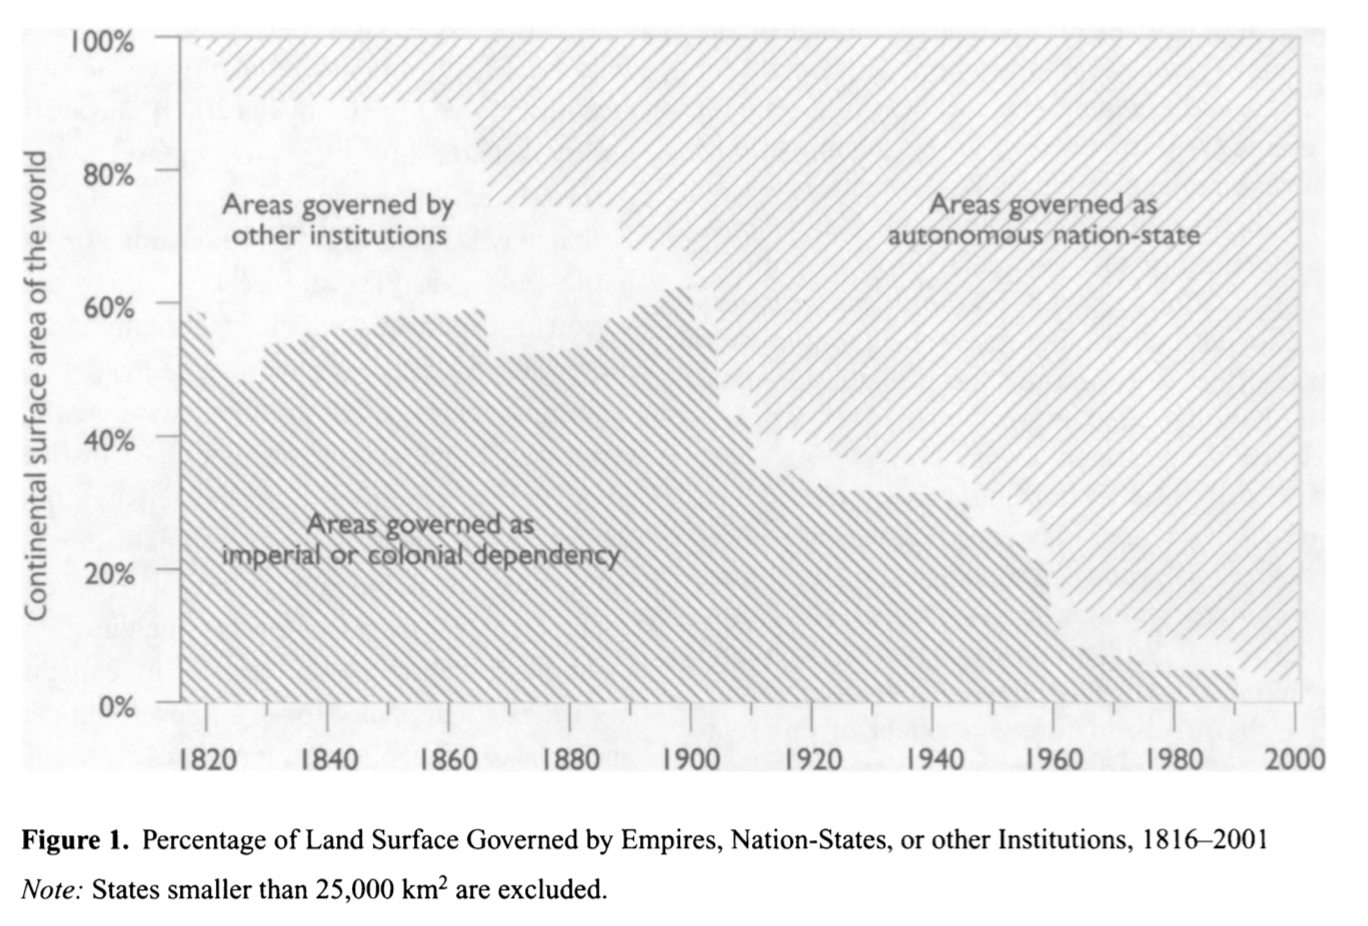
\includegraphics[width = \textwidth]{img/wimmer_min_fig1}

{\scriptsize \textit{Source:} Wimmen \& Min (2006)}

\end{frame}

\begin{frame}
\frametitle{Why war?}
\centering

\begin{itemize}[<+->]
  \item \textit{Competing} models of state building
  \item Wars not because of changes to the international balance (as in Waltz), but because of internal processes and competing claims to the same territory or population
  \item Creating an empire will cause resistance to incorporation, particularly in the peripheries
  \item Formation of nation-states leads to the violently reordering of states (inter-state wars) or, once they are formed, wars over internal power distribution
\end{itemize}

\end{frame}


\begin{frame}
\frametitle{Institutional changes and wars}
\centering

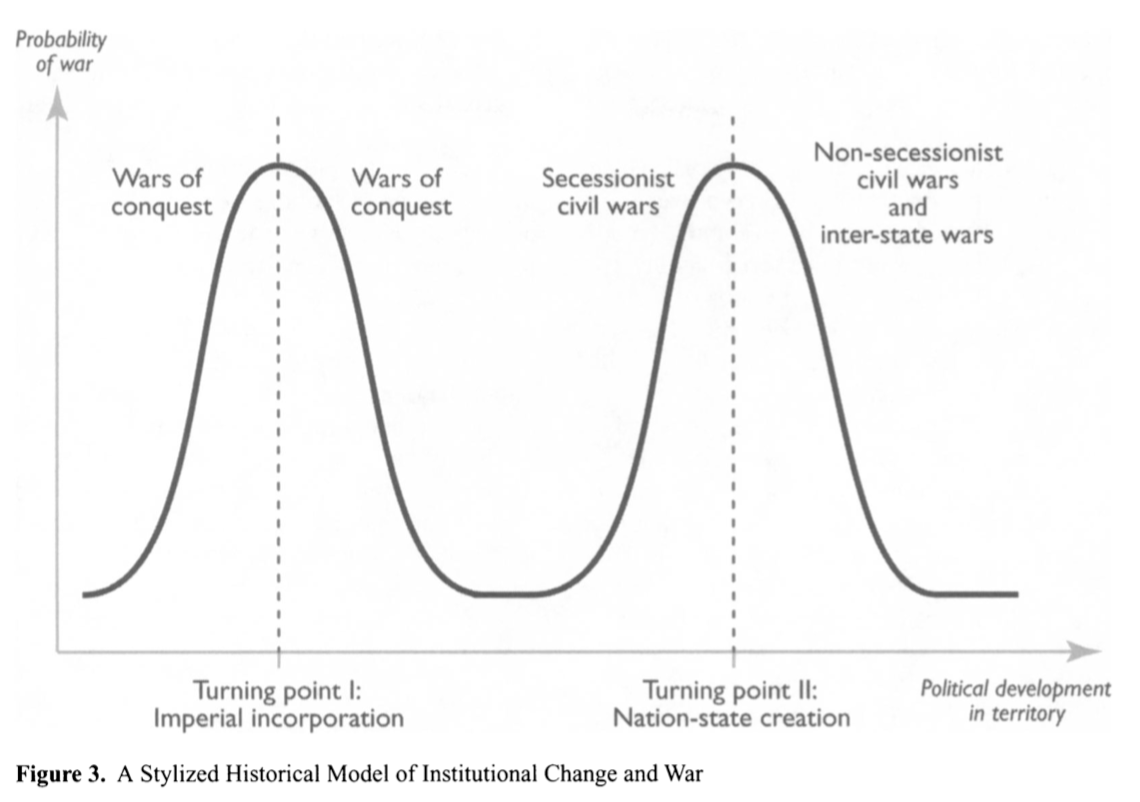
\includegraphics[width = 0.85\textwidth]{img/wimmer_min_fig3}

{\scriptsize \textit{Source:} Wimmen \& Min (2006)}

\end{frame}

\begin{frame}
\frametitle{Nation-states and wars}
\centering

\begin{itemize}[<+->]
  \item The rise of nationalism and nation-states in the world linked to different types of war
  \item Creating a nation-state often involves splitting off from a former polity: secessionist wars
  \begin{itemize}
    \item Many conflicts throughout the world (e.g. ETA in Spain)
  \end{itemize}
  \item Congruence between nations and states (nationalism) leads to irredentism wars
  \begin{itemize}
    \item Irredentism: from Italian \textit{irredento} (unredeemed), about territories inhabited by Italian-speaking populations ruled by the Austro-Hungarian empire during the 19th century
    \item E.g.: Ireland and Ulster, Nagorno-Karabakh?
  \end{itemize}
  \item Once nation-states are formed, conflicts over the distribution of power, ethno-political discrimination (civil wars)
\end{itemize}

\end{frame}

\begin{frame}
\frametitle{Nation-states and wars}
\centering

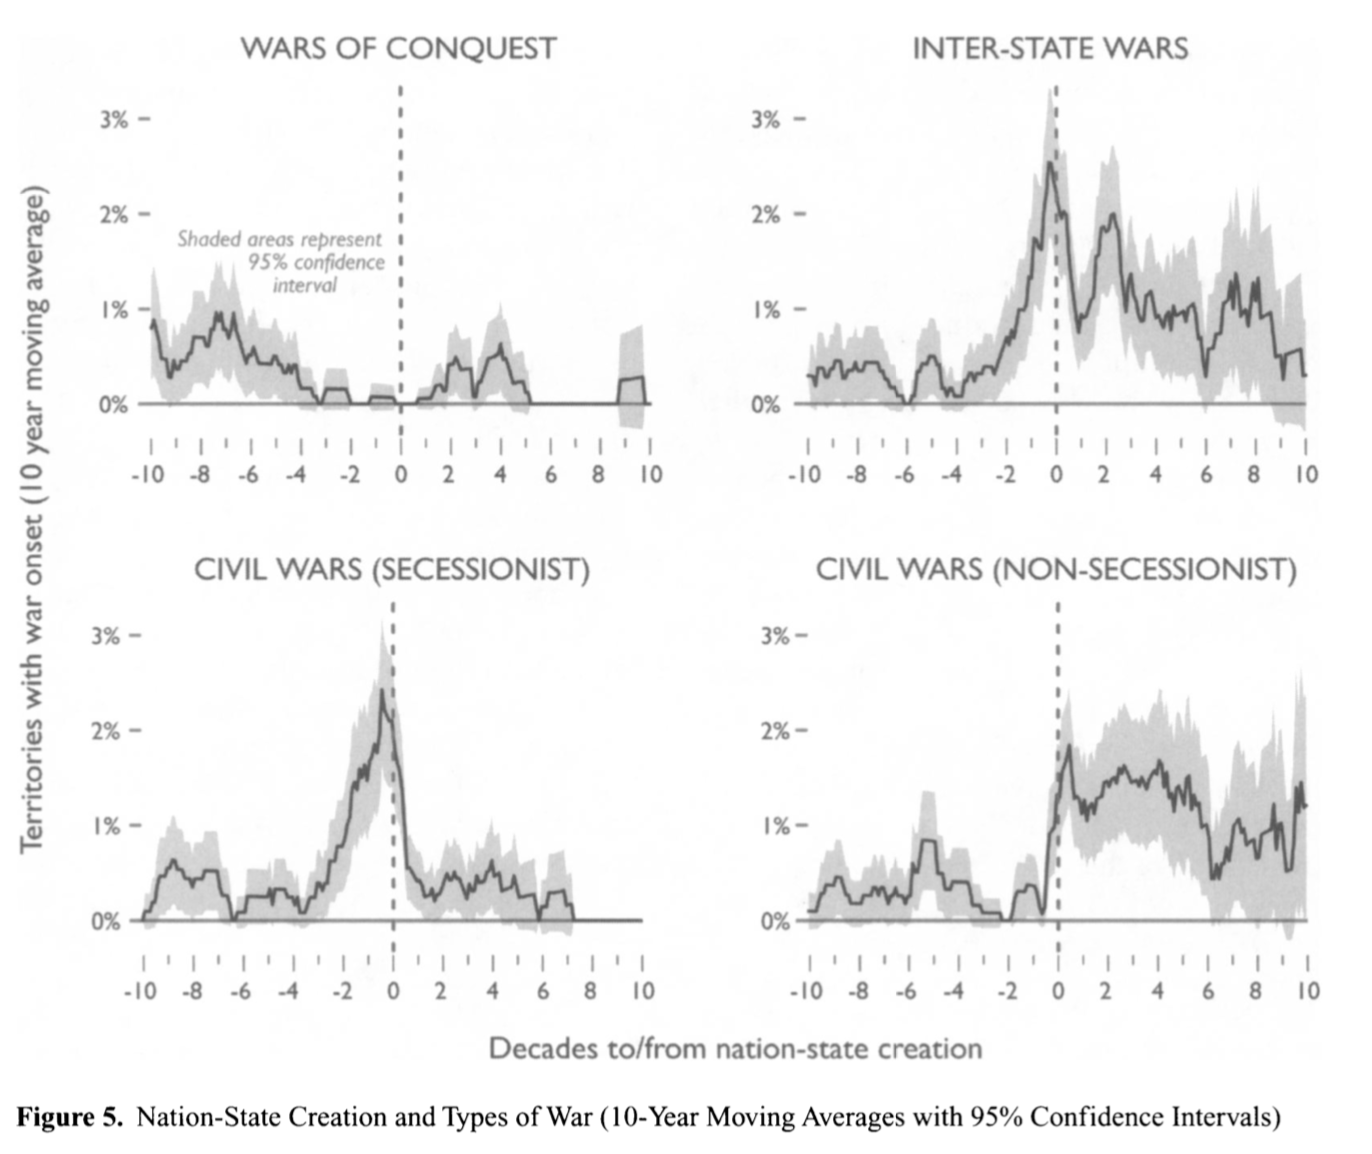
\includegraphics[width = 0.75\textwidth]{img/wimmer_min_fig5}

{\scriptsize \textit{Source:} Wimmen \& Min (2006)}

\end{frame}

\begin{frame}
\frametitle{Looking at the big picture}
\centering

\begin{itemize}
  \item Different type of questions:
  \begin{itemize}
    \item How did warfare evolve? How do changes to the international system impact overall levels of war?
  \end{itemize}
  \item $\neq$ explanations of political conflicts in particular
  \begin{itemize}
    \item explain the outbreak of individual conflicts, assess likelihood of a conflict in a given country
  \end{itemize}
  \item But these are macro-historical explanations: focus is on the evolution of warfare throughout history and what macro-level changes explain it
  \item Related to previous lecture on warfare and state formation
\end{itemize}

\end{frame}
% ----------------------------------------------------

\begin{frame}
\frametitle{Nationalism and internal conflict}
\centering

\begin{itemize}[<+->]
  \item Different perspective on nationalism and war: how it impacts specific internal conflicts
  \item Ethnicity $\neq$ nationalism
  \begin{itemize}
    \item Closely related concepts, sometimes (especially years ago) treated very differently
    \item Difference: claims of statehood (multi-ethnic nations, civic vs. ethnic nationalism, etc)
  \end{itemize}
  \item Early studies on ethnic conflict
  \begin{itemize}
    \item Almost no attention to the state, ethnic wars were seen as a conflict \textit{between} ethnic groups
    \item Ancient hatred idea, security dilemma, etc
  \end{itemize}
\end{itemize}

\end{frame}
% ----------------------------------------------------

\begin{frame}
\frametitle{Nationalism and internal conflict}
\centering

\begin{itemize}[<+->]
  \item Modern studies put emphasis on the role of state and political power
  \item Quantiative studies: role of grievances and ethnopolitical discrimination, etc (will see more on civil wars)
  \item External conflict: nation-to-state deficit and surplus
  \begin{itemize}
    \item If nations and states match, political stability
    \item State deficit: secessionist wars, etc
    \item Nation deficit: irredentism
    \item `Macedonian syndrome:' how nation-building spills off state borders and radicalizes host states, ethnic minorities, and irredentist states
  \end{itemize}
  \item Difference with previous macro-historical approach: looking at specific cases
\end{itemize}

\end{frame}
% ----------------------------------------------------

\begin{frame}
\frametitle{Making up the nation through violence}
\centering

\begin{itemize}[<+->]
  \item An ultimate version of the nation-to-state congruence: using violence to make up the nation
  \item Homogenizing policies: many available tools or strategies
  \item A last resort: ethnic cleansing or genocide
  \item Essentially a modern phenomenon, not about ancient barbarism
  \item Zygmunt Bauman's \textit{Modernity and Holocaust}
  % \item bulutgil etc
\end{itemize}

\end{frame}
% ----------------------------------------------------

\begin{frame}
\frametitle{Next Thursday}
\centering

\begin{itemize}
  \item `When constitutions took over the world'
  \item[] (Jill Lepore, \textit{The New Yorker})
  \item[]
  \item Nationalism $\rightarrow$ warfare
  \item Warfare $\rightarrow$ internal rule
  \item Q: changes in the source of sovereignty after rise of nationalism, and how they impact the use of political violence for internal rule (i.e. how problematic is ethnic diversity when you are playing the democratic game)
\end{itemize}

\end{frame}
% ----------------------------------------------------



\end{document}
